\documentclass[a4paper, 12pt]{article}

\usepackage[portuges]{babel}
\usepackage[utf8]{inputenc}
\usepackage[outline]{contour}
\usepackage[dvipsnames]{xcolor}
\usepackage{mathtools} % loads amsmath
\usepackage{amsmath}
\usepackage{amssymb}
\usepackage{indentfirst}
\usepackage{graphicx}
\setlength{\jot}{8pt}
\usepackage[colorinlistoftodos]{todonotes}


\begin{document}

\begin{titlepage}
	\begin{center}
		\huge{Anotações sobre a Iniciação Científica}

		\vspace{30pt}
		
	\end{center}
	
	\begin{flushleft}
		%\begin{tabbing}
		%	Alunos\qquad\qquad\= \>Heitor Barroso Cavalcante - 12566101\\\\
		%	Professora\> Nina S. T. Hirata \\
		%
	    %\end{tabbing}
		Aluno\qquad\qquad Heitor Barroso Cavalcante - 12566101\\
		\vspace{10pt}
		Professora \quad Nina S. T. Hirata \\
		  
	\end{flushleft}
	\vspace{30pt}
	\begin{center}
		21 de Abril de 2022
	\end{center}
	\tableofcontents
\end{titlepage}
%%%%%%%%%%%%%%%%%%%%%%%%%%%%%%%%%%%%%%%%%%%%%%%%%%%%%%%%%%%\\
\thispagestyle{empty}

\newpage
\pagenumbering{arabic}

%%%%%%%%%%%%%%%%%%%%%%%%%%%%%%%%%%%%%%%%%%%%%%%%%%%%%%%%%
%%%%%%%%%%%%%%%%%%%%%%%%%%%%%%%%%%%%%%%%%%%%%%%%%%%%
\section{Processamento de Imagens Digitais}
\subsection{Introdução}
O processamento de imagens é uma subárea da disciplina de ``Processamento de Sinais", e essa subárea pode ser dividida em processamento digital ou analógico de imagens.
\begin{itemize}
    \item Processamento Analógico de Imagens:\\
    As imagens são manipuladas através da variação de sinais elétricos, o maior exemplo deste tipo de processamento é a imagem de televisão.
    \item Processamento Digital de Imagens:\\
    Consiste em desenvolver sistemas digitais para manipular imagens.
\end{itemize}

Nesse sentido, imagens podem ser compreendidas como um sinal bidimensional e pode ser definida como uma função \(f(x,y)\) tal que \((x,y)\) são as coordenadas de um pixel e \(f(x,y\) é o valor deste pixel. Assim, figuras visualizadas em um computador, por exemplo são matrizes de inteiros que variam de 0 a 255. As dimensões da imagem são as dimensões da matriz.
\\

Um sinal, pode ser definido como qualquer quantidade física medida através do tempo, do espaço ou qualquer outra dimensão. Logo, uma imagem digital pode ser caracterizada como um sinal de duas dimensões.
\\

A formação de uma imagem digital parte de um processo físico. A luz refletida pelos objetos fotografados é medida por diversos sensores e uma tensão contínua é gerada de acordo com a quantidade de luz captada pelos sensores. Agora, esse sinal analógico deve ser convertido para um digital. Para isso, amostragem e quantização são utilizadas para gerar a matriz de números que forma a imagem digital.
\\

Visão Computacional consiste no desenvolvimento de um sistema que consiga, a partir de uma imagem, gerar uma saída contendo informações sobre a imagem. Por exemplo, sistemas com reconhecimento facial.
\\

Por fim, resumindo, o processamento de sinais é muito importante para
o processamento de imagens. Sensores captam a luz do mundo físico, resultando em um sinal bidimensional que, após ser processado, forma uma imagem digital. Aí então esta imagem é manipulada através do processamento digital de imagens.

\subsection{Introdução à Sinais e Sistemas}
Primeiramente, definindo os termos chaves dessa seção:
\subsubsection{Sinais}
Em Engneharia elétrica, a medida fundamental para representação
de informações é chamada sinal. Um sinal poderia ter quaisquer dimensões
e ser de qualquer forma.
\begin{itemize}
	\item Sinais Analógicos:
    \\
	Um sinal analógico, medido através do tempo é um sinal contínuo.
	Eles são difíceis de analizar. Para representá-los, precisariamos de memória infinita.
	Isso ocorre pois a amostra é ``infinita''. Um exemplo é a voz humana ou $y = \sin(x)$.
	\item Sinais Digitais:
	\\
	São a apropriação dos sinais analógicos de uma maneira descontínua, valores discretos
	são utilizados para representar informações. Logicamente são menos precisos que sinais
	analógicos.
\end{itemize}
\subsubsection{Sistemas}
Um sistema é definido através dos tipos de sinais de entrada e dos tipos de sinais de saída
em relação aos quais o sistema funciona. Nesse caso, um sistema pode ser interpretado como o processo
de conversão de um sinal analógico para um sinal digital.
\\

Em tal tipo de conversão, há dois conceitos chave. Amostragem e Quantização.
Amostragem pode ser definido como o ato de tirar amostras do sinal isso ocorre no domínio da função que representa o sinal analógico.
Já Quantização pode ser definido como o ato de particionar os valores que a função pode assumir.


\section{Aplicações do Processamento de Imagens Digitais}
\begin{itemize}
	\item Restauração de imagens.
	\item Análise de imagens médicas.
  	\item Sensoriamento remoto.
   	\item Visão computacional.
    \item Reconhecimento de padrões.
    \item Processamento de vídeos.
    \item Análise de imagens microscópicas.
\end{itemize}

\section{Dimensões das Imagens}
Primeiramente, o conceito de dimensão define o número mínimo de pontos necessários para saber a posição de um objeto particular 
no espaço. No caso das imagens, sabemos que são bidimensionais. Altura e Largura. No caso de vídeos, podemos considerar o tempo como
 uma terceira dimensão e, por isso, podemos classificar esse tipo de imagens (vídeos) como 3D. Desso modo, podemos definir a imagem como
 uma função de duas variaveis.
 \begin{center}
	$f(x,y) = Imagem$
 \end{center}

 É interessante ressaltar que um filme pode ser considerado 3D. E, portanto, na realidade, um filme 3D seria 4D.

\section{Formação de Imagens em Câmeras}
Primeiro, é bom comentar sobre a formação de imagens no olho humano. A luz é refletida pelos objetos e é captada pelos olhos. Ao entrar no olho
a imagem fica invertida na retina. Então, o cérebro interpreta a imagem invertida e a ``desinverte''.
\subsection{Formação de Imagens em Câmeras Analógicas}
Nesse tipo de câmera, o filme --- uma tira plástica --- é revestida com halogeneto de prata. Essa substância reage com os fótons e forma
o negativo das imagens fotografadas.
\subsection{Formação de Imagens em Câmeras Digitais}
Nesse tipo de câmera, a formação das imagens se dá através do uso de um vetor de sensores CCD. CCD significa Charged Couple Devices.
Ou seja, dispositivo de carga acoplada, que é um sensor semicondutor que é sensível à imagem e a converte em um sinal elétrico. Há uma matriz
retangular desses sensores, em que cada um dos sensores corresponde à um pixel da imagem formada. Depois de cada sensor na matriz armazenar uma carga
a partir da incidência de fótons, tal carga é transformada em uma tensão que é convertida em informação digital. Isso ocorre em um sensor por vez.

\section{Mecanismos das Câmeras}
\subsection{Aperture - Abertura}
Como o próprio nome diz, é um orifício que permite a passagem da luz para dentro da câmera. Há lâminas que regulam o tamanho da abertura 
fazendo com que mais ou menos luz tenha acesso ao interior da câmera.
O efeito da abertura da câmera corresponde ao brilho da imagem fotografada
\subsection{Shutter - Obturador}
Podemos pensar no obturador como uma espécie de cortina que fica depois da abertura da câmera. Por trás do obturador está a matriz de 
dispositivos de carga acoplada. Assim que o obturador se abre a imagem é formada nessa matriz. Os efeitos do obturador dependem do tempo 
que a ele permanece aberto. Quanto mais tempo mais claridade haverá na imagem. Nesse sentido, dois conceitos chaves sobre esse mecanismo 
são o tempo e a velocidade. ``Shutter speed'' e ``Shutter time''. A velocidade representa quantas vezes o obturador se abriu ou se fechou, já o tempo 
representa o intervalo de tempo em que ele permanece aberto. É interessante ressaltar que há uma relação inversamente proporcional 
entre a velocidade e o tempo. Quanto mais velocidade, menor tempo e vice-versa. Uma aplicação importante da velocidade e do tempo do obturador é o ato de 
capturar imagens que se movimentam em alta velocidade. Assim, quanto menor for o tempo do obturador, melhor conseguiremos capturar imagens que se movem rapidamente.

\subsection{ISO}
O fator ISO representa a sensibilidade de uma câmera à luz. Quanto maior o número ISO de uma câmera, mais sensível ela é à luz. 
Contudo, há um sintoma colateral que se pronuncia quando o número ISO é elevado. Nesses casos, há mais ruído na imagem capturada.

\subsection{Conceito de Pixel}
O pixel é a unidade da imagem. Em uma imagem em gray-scale de 8 bits, cada pixel possui um valor de 0 a 255, que corresponde à intensidade 
da luz naquele ponto. Novamente, cada dispositivo de carga acoplada corresponde à um pixel.
\subsubsection{Cálculo do número total de pixels}
Para saber a quantidade de pixels em uma imagem, basta multiplicar as dimensões da matriz
\begin{center}
	$\#pixels = \#colunas \cdot \#linhas$
\end{center}
\subsubsection{Valores de pixels}
Sabemos que cada pixel possui somente um valor. Além disso, por definição, o valor $0$ significa ausência de luz.

\section{Transformação de Perspectiva}
De modo geral, um exemplo claro do que é perspectiva, é o fato de, através dos olhos humanos, ao vizualizar objetos menos distantes, 
esses aparentam ser maiores. Nesse sentido, a transformação de perspectiva é sobre a conversão de uma realidade tridimensional 
(altura, largura e profundidade) em um uma imagem bidimensional (altura e largura).

\subsection{Referencial - Frame of Reference}
\textcolor{red}{
	\large{ACHEI ESSA PARTE CONFUSA}
	\\
	Para analisar o mundo/imagem/cena tridimensional, precisamos de 5 referenciais --- ``frame of references'' --- sendo esses:
\begin{itemize}
	\item Objeto
	\item Mundo
 	\item Camera
 	\item Imagem
 	\item Pixel
\end{itemize}
}
\newpage
De qualquer maneira, essa transformação pode ser compreendida ao utilizarmos simpes conceitos de ótica e trigonometria. Observe:
\begin{figure}[!htbp]
	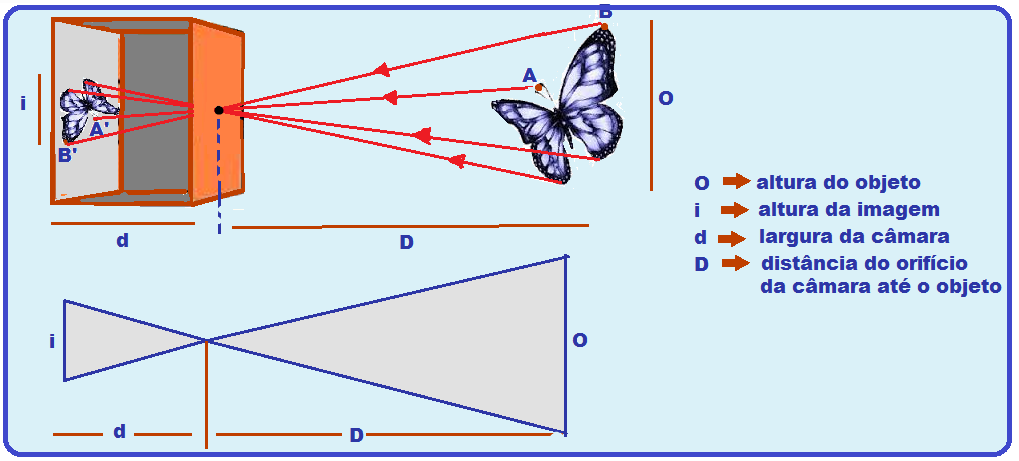
\includegraphics[scale=0.5]{images/otica.png}
	\caption{Imagem para exemplificar o uso da trigonometria na conversão do mundo 3D para o 2D}
\end{figure}
Podemos usar semelhança de triângulos para descobrir o tamanho da imagem formada $i$.
\begin{center}
	$\dfrac{i}{d} = \dfrac{O}{D} \Rightarrow i = d \dfrac{O}{D}$
\end{center}

\section{Conceito de bits por pixel}
O número de cores que podem ser representadas em uma imagem depende da quantidade de bits por pixel presente nessa imagem.
De maneira geral, podemos dizer que a maioria das imagens em gray-scale consiste de 8 bits por pixel. Equanto as coloridas tem, geralemente 
24 $bpp$. Isso pode ser compreendido ao imaginar que cada canal R, G, e B são possuem 8 bits.

Como dito anteriormente, o valor 0 é, por padrão, o valor que representa a cor preta, intensidade mínima em um canal de cor. 
Agora, o valor que representa o valor máximo não é padronizado, depende do $bbp$ dessa imagem. Então, teremos que esse valor pode ser 
representado por $2^{bpp} - 1$.

\subsection{Cálculo do tamanho (em memória) de uma imagem}
Para saber o tamanho de uma imagem, devemos levar em consideração as suas dimensões bidimensionais e o número de $bpp$. Por exemplo, digamos que 
uma imagem possua $1024$ linhas, $1024$ colunas e $8 bpp$, teremos:
\begin{center}
	$tamanho = 1024 \cdot 1024 \cdot 8 = 8388608 \; bits  \Rightarrow$ 
	\\
	\vspace*{0.15cm}
	$\Rightarrow tamanho = \dfrac{8388608}{8} = 1048576 \; bytes  \Rightarrow$ 
	\\
	$\Rightarrow tamanho = \dfrac{1048576}{1024} = 1024\;kb \Rightarrow tamanho = \dfrac{1024}{1024}\;Mb $
\end{center}

\section{Tipos de imagens}
\subsection{Imagem binária}
Nesse caso, há somente 2 valores possíveis para os pixels dessa imagem 0 ou 1. Onde 0 representa o preto e 1 o branco.
\begin{figure}[!htbp]
	\centering
	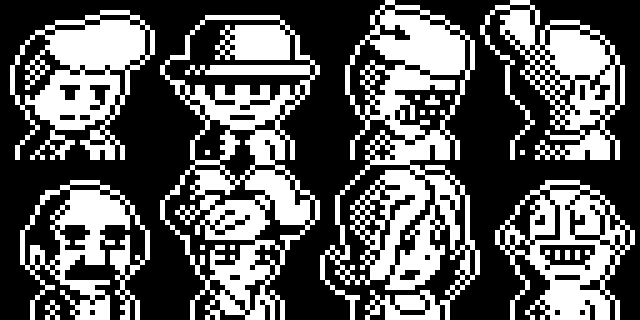
\includegraphics[scale=0.5]{images/binaria.png}
	\caption{Imagem binária}
\end{figure}
\subsection{Formato 8 bits de cor}
Comumente conhecida como imagens Grayscale.
\begin{figure}[!htbp]
	\centering
	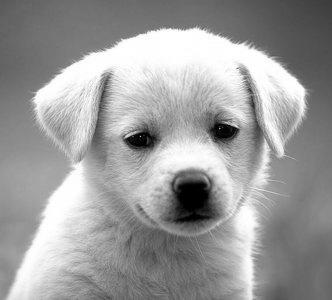
\includegraphics[scale=0.5]{images/grayscale.jpg}
	\caption{Imagem Grayscale}
\end{figure}

\subsection{Formato 16 bits de cor}
Aqui já temos imagens coloridas. Esses 16 bits são distribuídos nos 3 canais R, G e B. Da seguinte maneira:
\begin{itemize}
	\item 5 bits para o vermelho (R).
 \item 6 bits para o azul (G).
 \item 5 bits para o verde (B).
\end{itemize}

\subsection{Formato 24 bits de cor}
Por fim, temos o formato de imagens mais comuns hoje em dia. Em que temos esses 24 bits distribuídos igualmente entre os canais R, G e B.
\begin{figure}[!htbp]
	\centering
	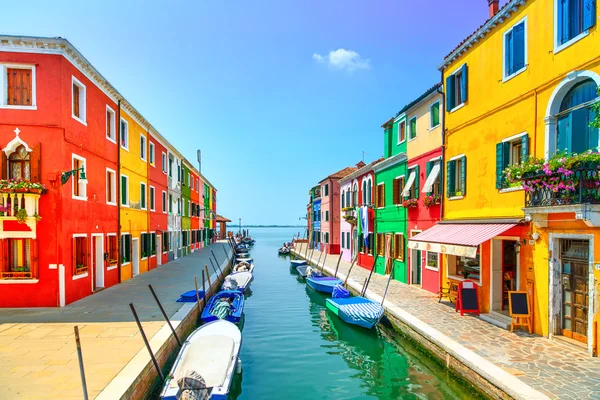
\includegraphics[scale=0.4]{images/colorida.png}
	\caption{Exemplo de imagem de 24 bits}
\end{figure}

\section{Códigos de cores}
Consideramos aqui que todas as cores estão no formato de 24bits. ou seja, uma cor ``$C$'' é tal que $(R, G, B) = (C_R, C_G, C_B)$
Assim, no formato RGB, temos:
\begin{itemize}
	\item \contour{black}{\textcolor{white}{Branco}} = (255, 255, 255)
 \item Preto = (0, 0, 0)
 \item \textcolor{red}{Vermelho} = (255, 0, 0)
 \item \textcolor{green}{Verde} = (0, 255, 0)
 \item \textcolor{blue}{Azul} = (0, 0, 255)
 \item \textcolor{gray}{Cinza} = (128, 128, 128)
		\\
		Nesse caso, a cor cinza é sempre o ponto médio entre a intensidade máxima e mínima. Logo, poderíamos escolher o valor 
		de 127 ou de 128. Nesse caso, escolhemos 128 (em todos os canais).
\end{itemize}

\subsection{Modelo CMYK}
Agora, vale ressaltar o modelo de cores CMYK --- comum em impressoras ---, aqui, CMYK significa ``cyan, magenta, yellow, black''. No conceito de impressoras,
geralmente há um cartucho de cores, (CMY) e outro preto. Assim, as cores ciano, magenta e amaerlo podem ser formadas ao se variar as porções de 
vermelho, verde e azul também. Os códigos RGB dessas cores são como segue.

\begin{itemize}
 \item \textcolor{magenta}{Magenta} = (255, 0, 255)
 \\
 Combinação de vermelho e azul.
 \item \textcolor{cyan}{Ciano} = (0, 255, 255)
 \\
 Combinação de verde e azul.
 \item \textcolor{yellow}{Amarelo} = (255, 255, 0)
 \\
 Uma combinação de vermelho e verde.
\end{itemize}

Além disso, também há o formato hexadecimal para representação de cores. Logo, para converter de um formato para outro, de RGB para hexadecimal ou 
vice versa, fazemos:

\subsection{Conversão RGB para Hexadecimal}
O formato de uma cor em hexadecimal é tal que \#FFFF00 (amarelo). para obter esses valores hexadecimais, deve-se, canal a canal RGB de uma dada cor, 
realizar a divisão do valor do canal por 16. Então, o quociente da divisão do canal R é o primeiro caracter do código, o segundo caracter 
é o resto dessa divisão. O terceiro valor é o quociente da divisão do valor do canal B por 16, o quarto é o resto dessa divisão. E assim por diante.
Observe:
\\
Sabemos que o código do \textcolor{yellow}{amarelo} é (255, 255, 0). Então, sobre R: $255/16$ tem quciente 15 e resto 15. FF. O mesmo ocorre com G. 
Agora, sobre B, teremos 00. Formando, assim o código \#FFFF00.

\subsection{Conversão Hexadecimal para RGB}
Para fazer o caminho inverso, devemos dividir o código hexadecimal em três porções. Sobre o exemplo do amarelo, temos FF, FF, 00. Agora, em um desses pares 
por vez, convertemos cada um de seus caracteres para binário. Concatenamos os dois números binários obtidos, convertemos para decimal e, assim, obtemos os valores dos canais. Observe: 
\\
Primeiramente, tratando de FF. convertendo para binário, temos 1111 e 1111. Concatenando: 11111111. Convertendo para decimal: 255 (valor do canal R)
Repetindo esses passos para os outros dois canais, obtemos o código da cor em (R, G, B).

\section{Conversão de RGB para Grayscale}
Primeiramente a maneira mais simples de se converter uma imagem para Grayscale é fazer a média entre os valores dos canais R, G e B.
\begin{figure}[!htb]
	\centering
	\minipage{0.30\textwidth}
	  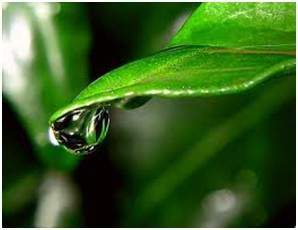
\includegraphics[width=\linewidth]{images/rgb.jpg}
	  \caption{Imagem original.}
	\endminipage\hspace{1cm}
	\minipage{0.30\textwidth}
	  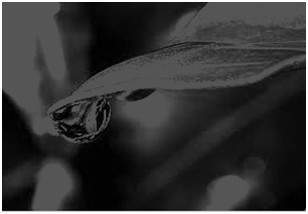
\includegraphics[width=\linewidth]{images/avg_gray.jpg}
	  \caption{Imagem Grayscale feita com a média}
	\endminipage
\end{figure}
Observe que essa figura não fica com um aspecto muito bom, fica ``empretecida''. Isso ocorre pois o olho humano não capta os níveis 
de vermelho, verde e azul na mesma proporção. Na realidade, o olho humano é muito mais sensível ao verde. Então, há o método de utilizar pesos para 
corrigir essas imperfeições. Então, se usarmos $30\%$ para o vermelho, $59\%$ para o verde e $11\%$ para o azul, teremos:

\begin{figure}[!htb]
	\centering
	\minipage{0.30\textwidth}
	  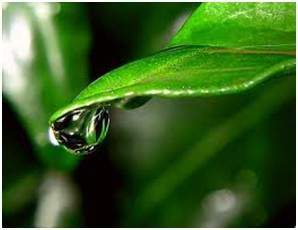
\includegraphics[width=\linewidth]{images/rgb.jpg}
	  \caption{Imagem original.}
	\endminipage\hspace{1cm}
	\minipage{0.30\textwidth}
	  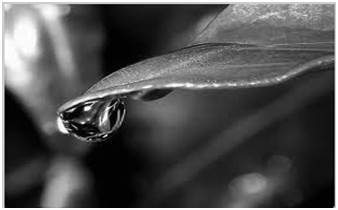
\includegraphics[width=\linewidth]{images/weighted_gray.jpg}
	  \caption{Imagem Grayscale feita utilizando pesos}
	\endminipage
\end{figure}


\section{Amostragem - Sampling}

Como dito anteriormente, o conceito de amostragem se relaciona ao processo de conversão de um sinal analógico para o digital. Assim, 
tiramos amostras do domínio da função que queremos converter. Logo, podemos correlacionar esse conceito com os pixels da imagem que será formada.
Imagine que queremos formar uma imagem de dimensões $5 \times 5$. Então, teremos que fazer uma amostragem da altura e largura do mundo que queremos representar 
em 5 valores diferentes cada. Ou seja, se a imagem é $f(x, y)$, $x$ assumirá 5 valores e $y$ assumirá 5 valores também. De maneira análoga, podemos 
relacionar esse conceito à matriz de dispositivos de carga acoplada ``CCDs''.

\subsection{Diferenças entre Zoom Analógico e Digital}
Apesar de ambos os conceitos se relacionarem ao fato de aumentarmos a amostragem do sinal, o zoom analógico aumenta essa amostragem através do movimento das lentes 
da câmera. Já o zoom digital funciona como se a imagem já houvesse sido capturada. Zoom analógico é feito nos sinais e o digital em uma imagem digital.

\section{Resolução de pixels}
De maneira simples, a resolução de uma imagem pode ser definida como a resolução a partir da qauntidade de pixels em uma imagem. Quando sabemos que a resolução de 
uma imagem é tal que $m \times n$ isso quer dizer que há $m$ colunas de pixel (largura) e $n$ linhas de pixel (altura). Nesse sentido, podemos calcular os 
MegaPixels de uma imagem fazendo $\dfrac{m \cdot n}{1\; mi}$ além disso, podemos saber o tamanho da imagem a partir de sua resolução também: 
$tamanho = pixelResolution \cdot bpp$ 

\subsection{Proporção da Tela}
Essa proporção nada mais é que a razão entre a largura da imagem e sua altura. Isso é extremamente útil ao mudar o tamnho das imagens, pois, 
se manetermos essa razão, então a imagem com tamanho modificado terá o mesmo aspecto que a imagem original.

\section{Mais sobre Zoom}
Como introduzimos os conceitos de zoom digital e analógico, podemos compará-los melhor. De fato, como o zoom analógico, ou óptico, nos proporciona 
um resultado melhor que o zoom digital. Isso ocorre pois, de fato estamos mudando a maneira como a fotografia será tirada, através do movimento das lentes.
Agora, o zoom digital, é simplesmente, aumentar uma certa área de vizualização de uma imagem, fazendo os pixels ficarem ``maiores''. Por isso, a qualidade da 
imagem é comprometida. Para fazer isso, há alguns métodos possíveis. ``Nearest neighbor interpolation'', ``Zero oeder hold method'', ``Zooming K times''.
\\

Um adendo interessante, é que o Exercício Programa 2 da disciplina de Laboratório de Métodos Numéricos, ministrada no primeiro semestre de 2022, tratou exatamente deste tópico.
Podemos considerar o ato de dar zoom em uma imagem com uma maneira de interpolar pontos, formando novos pixels a partir de pixels dados. Nesse sentido, estudamos os métodos de interpolação 
polinomial bilinear e bicúbica. Agora, continuemos a tratar dessas outras maneiras de dar zoom, que são abordadas no material.
\\

\subsection{Nearest Neighbor - Pixel Replication}
Para efetuar esse tipo de interpolação, devemos pensar, separadamente nas linhas e nas colunas da matriz que representa a imagem. Digamos que queremos 
aumentar a imagem por um fator de zoom $x$. Assim, assumindo que a imagem inicial tenha dimensões $3 \times 3$, por exemplo, e $x = 2$, a imagem final terá dimensões $6 \times 6$.
Agora, seja essa imagem exmplificada pela matriz:
\begin{table}[!htbp]
\centering
$
\begin{bmatrix}
	10 & 4 & 22 \\
	2 & 18 & 7 \\
	9 & 14 & 25
\end{bmatrix}
$
\end{table}

Primeiramente, devemos normalizar a posição dos pixels da nova imagem em relação à imagem antiga, fazemos isso sobre as linhas e sobre as colunas, obtendo uma razão entre 
o número de linhas da imagem original e o número de linhas da nova imagem. Análogo, para colunas. Então, obtemos duas proporções sobre as dimensões das duas imagens. 
Agora, múltiplicamos os índices de cada elemento da nova imagem por essa proporção. Desse modo, atribuiremos o valor do elemento (na imagem original) que possua índice mais próximo ao que 
foi calculado. Observe no exemplo, onde queremos interpolar os pontos $P_1$ e $P_2$.

$
\begin{bmatrix}
	10 & 4 & 22 \\
	2 & 18 & 7 \\
	9 & 14 & 25
\end{bmatrix}
\Rightarrow 
\begin{bmatrix}
	P_1 &  x &  x & x & x  & x \\
     x   &  x & x &  P_2 & x & x \\
	 x	& x & x &  x  &  x  & x  \\
	 x	& x & x &  x  &  x  & x \\
	 x	& x &  x  &  x  & x & x \\
	 x	& x & x &  x  &  x  & x \\
	 x	& x & x & x  & x  & x 

\end{bmatrix}$
Sabemos que a razão entre as linhas é: $\dfrac{3}{6} = \dfrac{1}{2}$ e as colunas a mesma. Então, o ponto $P_1$ tem coordenadas $(0, 0)$. 
Fazendo um produto escalar de $(0, 0)$ por $\left(\dfrac{1}{2}, \dfrac{1}{2}\right)$ teremos $(0, 0)$. O ponto $P_1$ tem ``vizinho mais próximo'' o pixel 
de coordenadas $(0, 0)$ na imagem original. $P_1 = 10$. Já em relação à $P_2$, teremos: $(1, 3) \cdot \left(\dfrac{1}{2}, \dfrac{1}{2}\right) = \left(0.5, 1.5\right)$. 
Tomando o teto: $(1, 2)$. O elemento $P_2$ tem vizinho mais próximo na imagem original o elemento de índice $(1, 2)$ e recebe seu valor. 
$P_2 = 7$. Fazendo o mesmo processo para todos os elementos, teremos a imagem com ``zoom'', ou seja, a imagem interpolada.
\begin{itemize}
\item Vantagem:
\\
É um processo extremamente simples.
\item Desvantagem:
\\
A imagem fica com um aspecto borrado.
\end{itemize}
Além disso, a imagem final terá tamanho tal que 
\\
$tamanhoFinal = \#linhasDaImagemOriginal \cdot fatorZoom \times \#colunasDaImagemOriginal \cdot fatorZoom$
\subsection{Zero-Order Hold - Bloqueio de Ordem Zero}
Esse algoritmo de zoom funciona de maneir muito simples. Para obter a imagem com zoom, devemos, colocar, entre os pixels da matriz da imagem original, 
pixels que tenham valores correspondentes à média dos seus vizinhos. Tome o exemplo:
\begin{center}
$
\begin{bmatrix}
1 & 2 \\
3 & 4
\end{bmatrix}
$
\end{center}
Inserindo uma linha entre as linhas dessa matriz, teremos:
\begin{table}
\centering
$
\begin{bmatrix}
1 & 1 & 2 \\
3 & 3 & 4
\end{bmatrix}
$
\end{table}

Observe que os valores insridos são o piso das médias obtidas. Agora, inserindo linhas entre as linhas:

\begin{table}
	\centering
	$
	\begin{bmatrix}
	1 & 1 & 2 \\
	2 & 2 & 3 \\
	3 & 3 & 4
	\end{bmatrix}
	$
\end{table}
Note que ocorreu o mesmo processo. A interpolação, ``zoom'' está feita.
\begin{itemize}
\item Vantagem:
\\
A imagem não fica com um aspecto borrado.
\item Desvantagem:
\\
Teremos que efeturar zoom nos baseando em potências de 2.
\end{itemize}

\subsection{K-times Zooming}
Esse algoritmo sana problemas dos que foram discutidos anteriormente. $K$ significa o fator de zoom.
Para explicar esse algoritmo, usaremos um exemplo. Tome a seguinte matriz como representação de uma imagem.
\begin{table}[!htbp]
	\centering
	$
	\begin{bmatrix}
	15 & 30 & 15 \\
	30 & 15 & 30
	\end{bmatrix}
	$
\end{table}
Primeiramente, supohemos $K = 3$. O número de valores que devem ser inseridos entre cada coluna e cada linha é $K - 1 = 3 - 1 = 2$.
Assim, iniciando pelas linhas (inserindo elementos entre as colunas) da matriz, temos que tomar os dois primeiros pixels 
adjacentes. ($15$ e $30$).
Subtraímos $15$ de $30$ ($15$). Dividimos o resultado da subtração por $K$ ($15/3 = 5$). Esse resultado é chamado de OP.
Agora devemos adicionar OP ao menor dos dois pixels escolhidos inicialmente ($5 + 15 = 20$) esse será o primeiro valor 
a ser inserido na matriz. Somamos OP a esse último resultado ($OP + 20 = 5 + 20 = 25$) e esse será o segundo elemento a ser
inserido na matriz, note que é o elemento de número $k - 1 = 2$ que foi inserido entre os dois primeiros elementos da primeira 
linha da matriz. Devemos fazer isso para todas as colunas. Ao fim desse processo, teremos a matriz:
\begin{table}[!htbp]
	\centering
	$
	\begin{bmatrix}
	15 & 20 & 25 & 30 & 20 & 25 & 15 \\
	30 & 20 & 25 & 15 & 20 & 25 & 30
	\end{bmatrix}
	$
\end{table}
\\
Depois de fazer isso, devemos ordenar os pixels inseridos de acordo com a ordem estaelecida na matriz. Por exemplo, no trecho:
$\begin{bmatrix}
	30 & \textcolor{blue}{20} & \textcolor{blue}{25} & 15	
\end{bmatrix}
$
\\
Tivemos os elementos em \textcolor{blue}{azul} inseridos. Note que a ordem da matriz era decrescente, da esquerda para a direita, indo 
de $30$ indo até $15$. Então, ordenaremos $\textcolor{blue}{20}$ e $\textcolor{blue}{25}$ em ordem decrescente também. Desse modo, 
Obteremos a seguinte matriz:
\begin{table}[!htbp]
	\centering
	$
	\begin{bmatrix}
	15 & 20 & 25 & 30 & 25 & 20 & 15 \\
	30 & 25 & 20 & 15 & 20 & 25 & 30
	\end{bmatrix}
	$
\end{table}
\\

Agora, precisamos efetuar o mesmo processo entre as linhas da matriz. Teremos:
\begin{table}[!htbp]
	\centering
	$
	\begin{bmatrix}
		15 & 20 & 25 & 30 & 25 & 20 & 15 \\
		20 & 21 & 21 & 20 & 21 & 21 & 20 \\
		25 & 22 & 22 & 25 & 22 & 22 & 25 \\
		30 & 25 & 20 & 15 & 20 & 25 & 30
	\end{bmatrix}
	$
\end{table}
Observe que usamos o piso da divisão de $5$ por $3$, e obtemos OP igual a $1$.

\large{\textcolor{red}{FIQUEI CONFUSO AQUI. O TUTORIAL DIZ QUE A IMAGEM FINAL FICA ASSIM, MAS EU NÃO TERIA QUE ORDENAR OS ELEMENTOS 
QUE FORAM INSERIDOS NOVAMENTE?}}

As dimensões da imagem final serão: $(K(\#linhas - 1) + 1) \times (K(\#colunas - 1) + 1)$

\begin{itemize}
	\item Vantagens:
 	\\
	Esse algoritmo combina as qualidades dos dois msotrados anteriormente. Não temos restrições quanto às dimensões da imagem final 
	e a imagem não fica muito borrada.
	\item Desvantagens:
 	\\
	Devido à necessidade de ordenação, esse algoritmo fica computacionamente mais custoso que os demais.
\end{itemize}

\section{Resolução Espacial - Spatial Resolution}
Esse tipo de resolução se relaciona ao menor detalhe que pode ser identificado em uma imagem. Podemos definir essa resolução também como 
o número de pixels independentes por polegada. Em suma, esse conceito se refere à comparação de imagens de uma mesma resolução (mesmas 
dimensões) para saber qual possui mais nitidez. Observe:
\begin{figure}[!htb]
	\centering
	\minipage{0.30\textwidth}
	  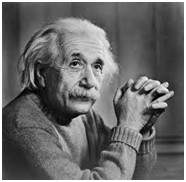
\includegraphics[width=\linewidth]{images/einsteinNitido.jpg}
	  \caption{Imagem com maior resolução espacial}
	\endminipage\hspace{1cm}
	\minipage{0.30\textwidth}
	  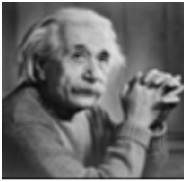
\includegraphics[width=\linewidth]{images/einstein_spatial.jpg}
	  \caption{Imagem com menor resolução espacial}
	\endminipage
\end{figure}
Podemos medir esse tipo de resolução das seguintes maneiras:
\begin{itemize}
	\item Pontos por Polegada.
 	\item Pixels por Polegada.
\end{itemize}

\subsection{Pixels por Polegada}
Geralmente usada para medir qualidade de telas, sabemos que, para obter essa unidade, devemos, primeiramente, 
obter a diagonal em pixels do visor calculada, a partir de sua resolução em pixels. $c = \sqrt[]{altura^2 + largura^2}$
Depois disso, dividiremos essa diagonal em pixels pelo tamanho da diagonal. $PPi = c/diagonalPolegadas$.

\subsection{Pontos por Polegada}
Essa unidade é, geralmente, utilizada para representar a qualidade de impressoras. Isto é, mede quantos pontos de tinta são impressos 
por polegada.

\section{Resolução Grayscale}
Resgatando conceitos já tratados anteriormente, a resolução em Grayscale tem íntima relação com a medida de $bpp$ (bits por pixel). Ou seja, 
quanto mais nuances de cinza puderem ser representadas, maior a resolução dessa imagem em termos de grayscale. Ainda, o total de nuances de cinza 
que podem ser exibidas nessa imagem com $bpp = k$ é tal que $2^k$, mas podemos também representar essa resolução puramente pelo número de 
$bpp$ e não pela quantidade de nuances de cinza que esse número produz.

\section{Conceito de Quantização}
Já sabemos que, no processo de conversão de um sinal analógico para um digital, há os conceitos de amostragem e quantização. Amostragem é 
feita no domínio do sinal, ou função. Já a quantização, é realizada nos valores que a função pode assumir. Ou seja, na imagem dessa função, feita no eixo 
$y$. Na realidade, ao quantizar um sinal, estamos digitalizando as amplitudes desse sinal, as particionando. Nesse sentido, podemos interpretar a resolução 
grayscale de uma imagem como um exemplo de quantização. Ao limitar os valores de cor que a imagem pode assumir, estamos quantizando as amplitudes do sinal.
Então, observe as diferenças entre Imagens com diferentes níveis de resolução grayscale (quantizações distintas).
\begin{figure}[!htb]
	\centering
	\minipage{0.17\textwidth}
	  	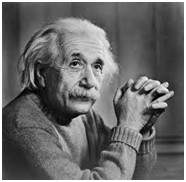
\includegraphics[width=\linewidth]{images/einstein256.jpg}
	  	\caption{256 níveis de cinza.}
	\endminipage\hspace{1cm}
	\minipage{0.17\textwidth}
	 	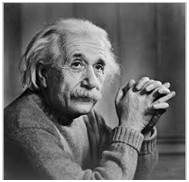
\includegraphics[width=\linewidth]{images/128.jpg}
	  	\caption{128 níveis de cinza.}
	\endminipage\hspace{1cm}
	\minipage{0.17\textwidth}
		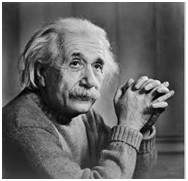
\includegraphics[width=\linewidth]{images/64.jpg}
		\caption{64 níveis de cinza.}
  	\endminipage\hspace{1cm}
  	\minipage{0.17\textwidth}
  		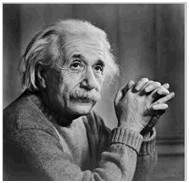
\includegraphics[width=\linewidth]{images/32.jpg}
  		\caption{32 níveis de cinza.}
	\endminipage
\end{figure}
\\
\begin{figure}[!htb]
	\centering
	\minipage{0.17\textwidth}
	  	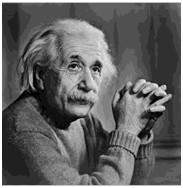
\includegraphics[width=\linewidth]{images/16.jpg}
	  	\caption{16 níveis de cinza.}
	\endminipage\hspace{1cm}
	\minipage{0.17\textwidth}
	 	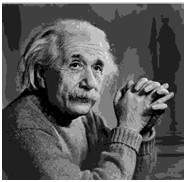
\includegraphics[width=\linewidth]{images/8.jpg}
	  	\caption{8 níveis de cinza.}
	\endminipage\hspace{1cm}
	\minipage{0.17\textwidth}
		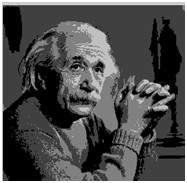
\includegraphics[width=\linewidth]{images/4.jpg}
		\caption{4 níveis de cinza.}
  	\endminipage\hspace{1cm}
  	\minipage{0.17\textwidth}
  		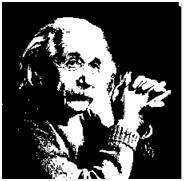
\includegraphics[width=\linewidth]{images/2.jpg}
  		\caption{ níveis de cinza.}
	\endminipage
\end{figure}

\section{Curvas de Preferência ISO - ISO Preference curves}
Como podemos observar nas imagens acima, a partir de uma certa quantidade de níveis de cinza, há o aparecimento de linhas na imagem. 
Tais linhas são chamadas de ``countouring''. Note que quanto mais discretizarmos (maior quantização) a imagem, mais aparecem essas linhas.
Contudo, esse não é o único fator que influencia no ``countouring''.
\subsection{Curvas de Isopreferência}
Em suma, estudos comprovaram que o aparecimento das linhas características do ``countouring'' está também relacionado à quantidade de detalhes presentes 
na imagem. Isso quer dizer que quanto mais detalhes uma imagem tiver, mais demorará para o efeito do ``countouring'' se tornar evidente.

\section{Conceito de Dithering \textcolor{red}{ACHEI ESSA SEÇÃO CONFUSA}}
Dithering é uma forma de ruído digital aplicado intensionalmente em um sinal. Nesse sentido, podemos ``permutar'' os pixels de uma imagem com baixos níveis de grayscale 
utilizando dithering para tornar mais detalhes visíveis nessa imagem.
\\

Primeiro, devemos trabalhar com limiares --- thresholding --- 

\section{Introdução a Histogramas}
\subsection{Histograma de uma Imagem}
O histograma de uma imagem mostra as frequências das intensidades dos pixels. Tomando, novamente, o exemplo de uma imagem grayscale, no eixo $x$, teremos 
as intensidades (níveis) de cinza presentes na imagem, enquanto no eixo $y$, teremos a frequência de ocorrência dessas intensidades.
\\
\begin{figure}[!htb]
	\centering
	\minipage{0.30\textwidth}
	  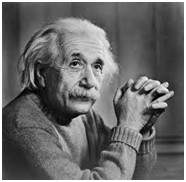
\includegraphics[width=\linewidth]{images/einsteinNitido.jpg}
	  \caption{Imagem}
	\endminipage\hspace{1cm}
	\minipage{0.30\textwidth}
	  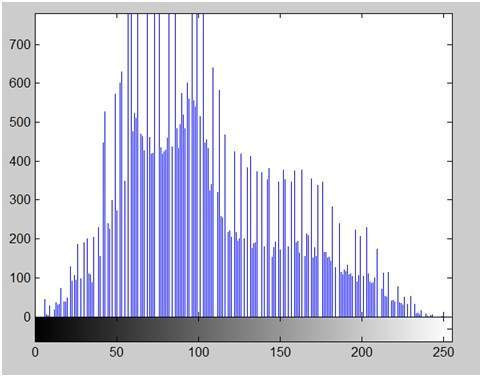
\includegraphics[scale=0.3]{images/histograma.jpg}
	  \caption{Histograma da Imagem}
	\endminipage
\end{figure}
\subsection{Aplicações dos Histogramas}
Uma das principais utilidades dos histogramas é a análise geral de imagens, podemos examinar uma imagem a partir de seu histograma. Além disso, 
estudar o brilho e contraste da imagem pode ser feito através do histograma. Por fim, há amplos usos em limiar --- thresholding ---, que são utilizados 
em visão computacional.

\section{Brilho e Contraste}
Brilho é um conceito relativo. Logo, podemos definir brilho como uma relação entre a quantidade de luz presente na saída (imagem) e 
a quantidade de luz presente na entrada (mundo real). Para tornar uma imagem mais ``clara'' (no sentido de possuir mais bilho ou luminosidade), basta adicionar 
valores à matriz que representa a imagem. Assim --- supondo uma imagem grayscale --- a cada vez que adicionarmos valores positivos à matriz, estaremos 
aproximando os valores de seus pixels à 255 (branco).

\subsection{Contraste}
Para definir contraste, simplesmente, podemos dizer que conceito corresponde à diferença máxima (em módulo) entre os valores dos pixels da matriz da imagem.
Então, se o valor máximo de um pixel em uma matriz em grayscale for, por exemplo, $200$ e o valor mínimo for $0$, teremos um contraste de $200$ nessa imagem.

\section{Transformação em imagens}
Inicialmente, é válido ressaltar que uma transformação é uma função que leva elementos de um conjunto à outro conjunto. Agora, sendo 
$f(x, y)$, a imagem de entrada, $G(x, y)$ a imagem de saída e $T(r)$ a função de transformação que ocorrerá na imagem, temos:
$G(x, y) = T(f(x, y))$.
\\
Exemplo:
\\

Considerando uma função de binarização da imagem, podemos considerar que, se um pixel ($f(x, y)$) possuir valor maior que $127$, deve se 
tornar branco e, caso contrário, deve se tornar preto. Então, podemos denotar que a função de transformação é tal que:
\begin{center}
	$T(f(x, y)) = 
	\begin{cases}
		1 \; se \; f(x, y) > 127 \\
		0 \; se \; f(x, y) \leq 127
	\end{cases}$
\end{center}

\section{Deslizamento de Histogramas - Histogram Sliding}
O conceito de ``delizar'' um histograma é, basicamente, mover o histograma de uma imagem para a direita ou para a esquerda. Desse modo, podemos usar esse ato 
para manipular o brilho de uma imagem. Intuitivamente, se quisermos aumetar o brilho de uma imagem, ao ``deslizar'' seu histograma para a direita, digamos, em 
$50$ valores, teremos, simplesmente adicionado o valor $50$ a todos os pixels da imagem, o que significa, exatmamente, aumentar o brilho da imagem. De maneira 
análoga, fazemos o oposto para diminuir o brilho de uma imagem (deslizamos o seu histograma para a esquerda).

\section{Alongamento de Histogramas - Histogram Stretching}
Outra operação que podemos fazer com histogramas, produzem alterações interessantes na imagem é o ``alongamento''. Ao fazer isso, alteramos o contraste da imagem.
Há diversar abordagens para realizar essa tarefa. Abordaremos com maior detalhe, uma transformação que se chama ``Min-Max Stretching'', ou seja 
esticamento mínimo-máximo.
\\

Nesse tipo de transformação, o valor mínimo de um pixel na imagem é mapeado para o valor $0$ e o valor máximo é mapeado para $255$. Os valores intermediários 
serão transformados de acordo com a fórmula: 
\begin{center}
$f(x,y)_{novo} = \dfrac{f(x, y) - f(x, y)_{min}}{f(x, y)_{max} - f(x, y)_{min}} \cdot 255$
\end{center}
Observe um exemplo dessa transformação:
\\
\begin{figure}[!htbp]
	\centering
	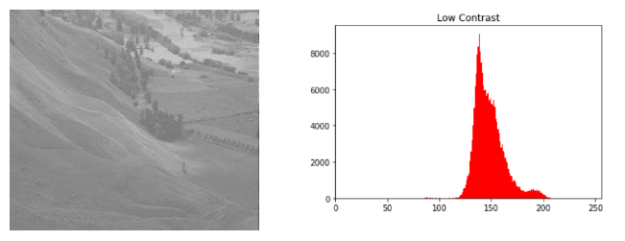
\includegraphics[scale=0.5]{images/origins.png}
	\caption{Imagem original}
\end{figure}
\\

\begin{figure}[!htbp]
	\centering
	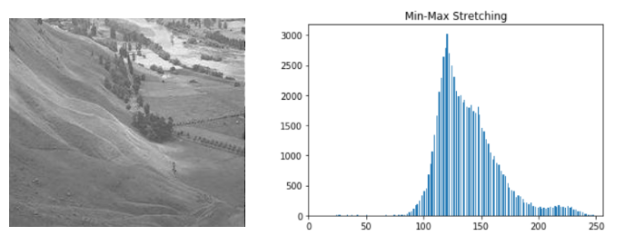
\includegraphics[scale=0.5]{images/minMax.png}
	\caption{Imagem original}
\end{figure}
\vspace{2cm}
Agora, como nessa maneira de ``esticar'' o histograma, levamos em consideração, simplesmente o maior e o menor valor, há a possibilidade de que valores outilers 
modifiquem o resultado final da imagem. Então, se retirarmos as bordas do histograma, ou seja, desconsiderarmos pixels que saiam do padrão de valores 
presentes na imagem, podemos melhorar o resultado final. Note que, nesse exemplo, há poucos pixels com valores menores que $100$, que, certamente atuaram para 
deixar a imagem transformada mais ``esbranquiçada''. Logo, se desconsiderarmos esses pixels, ``cortando'' o histograma, com certeza teremos um resultado final melhor.
Essa técnica é chamada de ``Percentile - Stretching''.

%https://theailearner.com/2019/01/30/contrast-stretching/

\begin{figure}[!htbp]
	\centering
	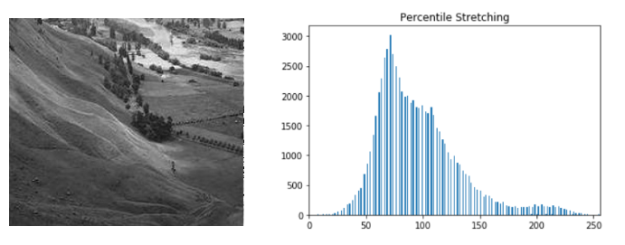
\includegraphics[scale=0.4]{images/percentile.png}
	\caption{Percentil histogram stretching}
\end{figure}

\section{Probabilidade para Transformações de Histogramas}
Uma operação muito importante que é efetuada em histogramas de imagens se chama equalização --- Histogram Equalization. Dessa maneira, para realizar tal 
operação, é necessário saber calcular a função de massa de probabilidade e a distribuição de probabilidade acumulada do histograma --- ou 
da própria imagem --- em questão. Logo, vamos 
comentar sobre esses dois conceitos de probabilidade.
\begin{enumerate}
	\item Função de massa de probabilidade:
    \\
	De maneira geral, essa função associa um valor de probabilidade à uma variável aleatória discreta (nesse caso, os valores dos pixels).
	Então, supondo a seguinte representação de uma imagem:
	\\

	\begin{table}[!htbp]
		\centering
		$
		\begin{bmatrix}
			0 & 1  & 50 \\
			2 & 30 & 0  \\
			2 & 1  & 1
		\end{bmatrix}
		$
	\end{table}
	Podemos montar a tabela de função de massa de probabilidade:
	\\

	\begin{center}
		\begingroup
		\renewcommand*{\arraystretch}{2.2}
		\begin{tabular}{|c|c|c|}
			\hline
			Valor do pixel & Frequência de aparecimento & $f(x)$     \\ \hline
			$0$            & $2$                        & $\dfrac{2}{9}$ \\ \hline
			$1$            & $3$                        & $\dfrac{3}{9}$ \\ \hline
			$2$            & $2$                        & $\dfrac{2}{9}$ \\ \hline
			$30$           & $1$                        & $\dfrac{1}{9}$ \\ \hline
			$50$           & $1$                        & $\dfrac{1}{9}$ \\ \hline
			\end{tabular}
		\endgroup
	\end{center}


		De maneira análoga, podemos calcular essa função de probabilidade a partir do histograma de uma imagem. Considere o seguinte histograma:
\begin{figure}[!htbp]
	\centering
	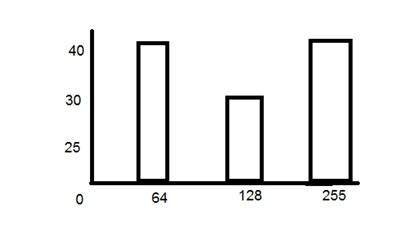
\includegraphics[scale=0.5]{images/hist1.jpg}
	\caption{Exemplo de histograma para FMP}
\end{figure}
		
		Note que o eixo $y$ desse histograma mostra as frequências de ocorrência dos valores dos pixels. Então, para cada valor que ocorre ($64$, $128$ e $255$), 
		basta calcular a razão entre suas ocorrências (frequência) e o total de valores presentes na imagem. Então, para este histograma, teremos a seguinte 
		função de massa de probabilidade:
		\\
		\begin{center}
			\begingroup
			\renewcommand*{\arraystretch}{2.2}
			\begin{tabular}{|c|c|c|}
				\hline
				Valor do pixel & Frequência de aparecimento & \begin{tabular}[c]{@{}c@{}}$f(x)$\end{tabular} \\ \hline
				$64$           & $40$                       & $\dfrac{40}{110}$                                        \\ \hline
				$128$          & $30$                       & $\dfrac{30}{110}$                                        \\ \hline
				$255$          & $40$                       & $\dfrac{40}{110}$                                        \\ \hline
				\end{tabular}
			\endgroup
		\end{center}
		 
	
	\item Função distribuição acumulada de probabilidade:
 	\\
	Esse conceito corresponde à soma acumulada das funções massa e probabilidade para cada valor do histograma, ou da imagem. Para exemplificar, 
	é válido obser var um gŕafico que represente essa função:

	\begin{figure}[!htbp]
		\centering
		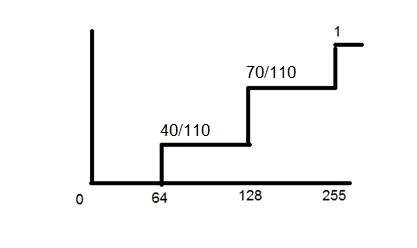
\includegraphics[scale=0.5]{images/prob3.jpg}
		\caption{Exemplo de histograma para FMP}
	\end{figure}
	
	Note, que, como a definição deixa claro, essa função corresponde à soma das funções de massa de probabilidade dos valores anteriores ao valor analisado 
	no momento. Ou seja, 
	\begin{center}
		\[F(x) = \sum_{xi<x}{f(x_i)} \]
	\end{center}
\end{enumerate}

\section{Equalização de Histogramas - Histogram Equalization}
Usaremos essa técnica de equalização de histogramas para aumentar o contraste de uma imagem. Contudo, em alguns casos, ao efetuar esse processo, 
o contraste da imagem pode acabar diminuindo.
\\

Desse modo, vamos explicar a partir de um exemplo. Considere que nossa imagem possua os seguintes valores de cinza e as respectivas funções acumuladas 
de probabilidade:

\begin{table}[!htbp]
	\centering
	\begin{tabular}{|c|c|}
	\hline
	Valor de cinza & CDF  \\ \hline
	0              & 0.11 \\ \hline
	1              & 0.22 \\ \hline
	2              & 0.55 \\ \hline
	3              & 0.66 \\ \hline
	4              & 0.77 \\ \hline
	5              & 0.88 \\ \hline
	6              & 0.99 \\ \hline
	7              & 1    \\ \hline
	\end{tabular}
\end{table}

Agora, efetuamos a seguinte operação: $\lfloor CDF \cdot (2^{bpp} - 1) \rfloor$ e adicionar à uma nova coluna, (nesse caso, temos 
$bpp = 3 \therefore 2^{bpp} = 9 \therefore 2^{bpp} - 1 = 7$) obtendo:

\begin{table}[!htbp]
	\centering
	\begin{tabular}{|c|c|c|}
	\hline
	Valor de cinza & CDF  & $\lfloor CDF \cdot (2^{bpp} - 1) \rfloor$ \\ \hline
	0              & 0.11 & 0                                     \\ \hline
	1              & 0.22 & 1                                     \\ \hline
	2              & 0.55 & 3                                     \\ \hline
	3              & 0.66 & 4                                     \\ \hline
	4              & 0.77 & 5                                     \\ \hline
	5              & 0.88 & 6                                     \\ \hline
	6              & 0.99 & 6                                     \\ \hline
	7              & 1    & 7                                     \\ \hline
	\end{tabular}
\end{table}

Esse valor que calculamos será o novo valor que os pixels que possuiam os antigos valores de cinza assumirão. Então, basta trocar os valores e obteremos 
uma imagem que teve seu histograma equalizado. Observe as mudanças:
\\

\begin{figure}[!htb]
	\centering
	\minipage{0.30\textwidth}
	  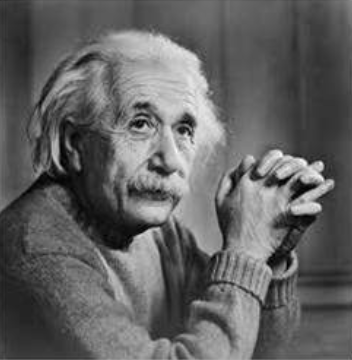
\includegraphics[width=\linewidth]{images/velho.png}
	  \caption{Imagem original}
	\endminipage\hspace{1cm}
	\minipage{0.30\textwidth}
	  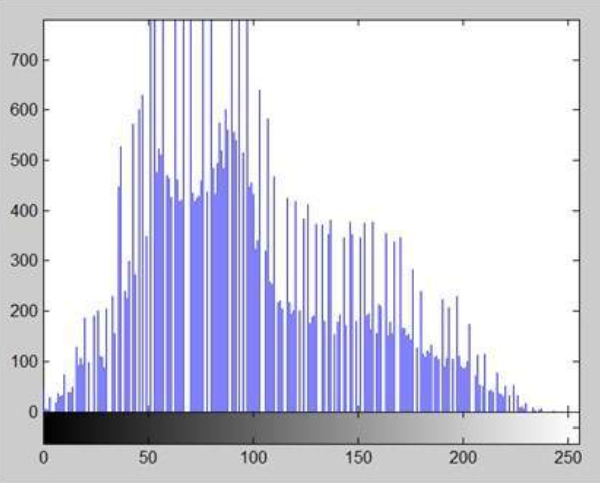
\includegraphics[scale=0.3]{images/velhoHist.png}
	  \caption{Histograma da Imagem original}
	\endminipage
\end{figure}

\begin{figure}[!htb]
	\centering
	\minipage{0.30\textwidth}
	  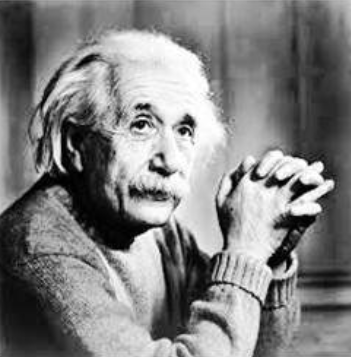
\includegraphics[width=\linewidth]{images/novo.png}
	  \caption{Nova imagem}
	\endminipage\hspace{1cm}
	\minipage{0.30\textwidth}
	  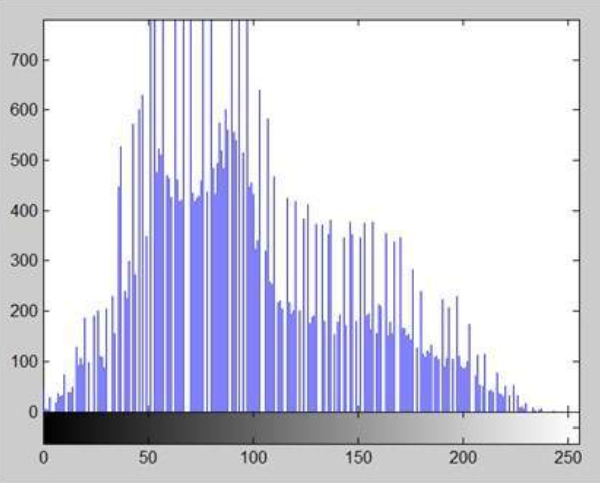
\includegraphics[scale=0.3]{images/velhoHist.png}
	  \caption{Histograma da nova imagem}
	\endminipage
\end{figure}
Podemos notar que o contraste aumentou na imagem produzida. Além disso, é válido mencionar que, com essa operação, o formato do histograma é distorcido, 
enquanto os esticamentos e deslizamentos de histograma mantem a forma original do histograma.

\section{Transformações de Níveis de Cinza}
\subsection{Aprimoramento de imagens}
Nesse contexto, o aprimoramento de imagens assegura um melhor contraste e maior nível de detalhes se comparado à uma imagem ``crua''. Isso pode ser 
feito por meio de transformações dos níveis de cinza dos pixels de uma imagem (grayscale).

\subsection{Transformação de Nível de Cinza}
Há três transformações básicas de níveis de cinza:
\begin{itemize}
	\item Linear 
 	\item Logarítimica 
  	\item Power - Law --- (Exponencial?)  
\end{itemize}

\subsubsection{Transformação Linear}
Como o nome diz, os valores de cada pixel na saída da transformação terão uma relação linear com os valores dos pixels de entrada. Nesse sentido, 
podemos evidenciar duas transformações lineares: 
\begin{enumerate}
	\item Transformação Identidade:
 	\\
	Nesse tipo de transformação, sendo $g(f(x,y))$ o valor de saída do pixel e $f(x, y)$ o valor de entrada, teremos:
	\begin{center}
		$g(f(x, y)) = f(x,y)$
	\end{center}
	
	Ou seja, a imagem de saída é exatamente igual à de entrada.

	\item Transformação Negativa:
 	\\
	Nesse tipo de transformação, seguindo os padrões estabelecidos no item imediatamente anterior, teremos:
	\begin{center}
		$g(f(x,y)) = 2^{bpp} - f(x,y)$
	\end{center}

	Note que, se $f(x, y)$ tem o valor do maior nível de cinza, $g(x,y)$ será zero e vice-versa. Estaremos produzindo a imagem negativa.
	\begin{figure}[!htb]
		\centering
		\minipage{0.30\textwidth}
		  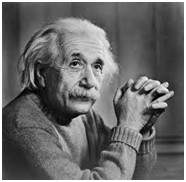
\includegraphics[width=\linewidth]{images/einstein256.jpg}
		  \caption{Imagem de entrada}
		\endminipage\hspace{1cm}
		\minipage{0.30\textwidth}
		  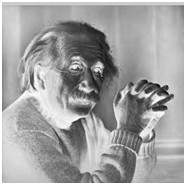
\includegraphics[scale=0.62]{images/graylevel4.jpg}
		  \caption{Imagem de saída}
		\endminipage
	\end{figure}
\end{enumerate}

\subsubsection{Transformação Logarítimica}
Há duas transformações logarítimicas principais, as logarítimicas de fato e as logarítimicas inversas. Explicaremos sobre as transformações 
logarítimicas e o inverso valerá para as inversas. Primeiramente, poderemos esperar uma padronização no aspecto da imagem. Isso ocorre devido à forma 
geral das funções logarítimicas (de acordo com o crescimento dos valores de $x$, os valores de $f(x,y)$ vão se aproximando).
\begin{figure}[!htbp]
	\centering
	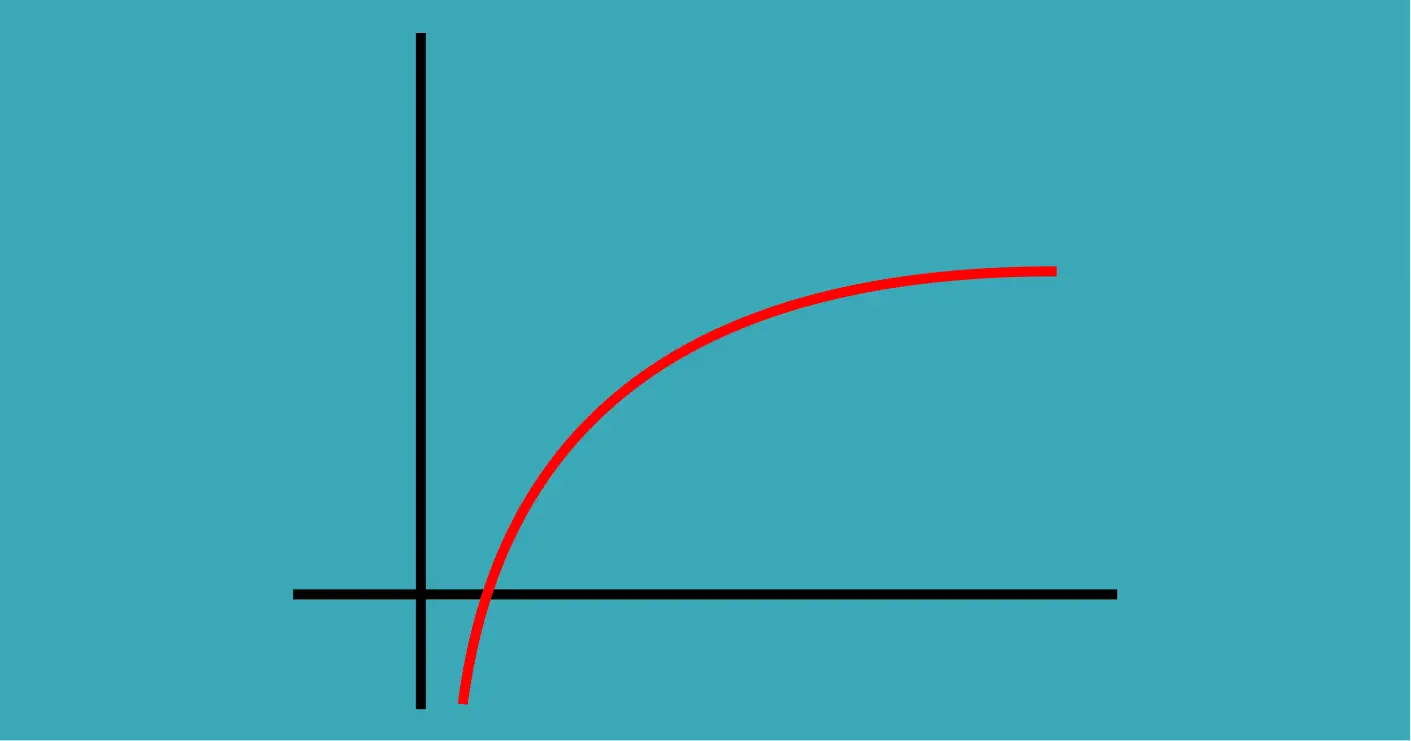
\includegraphics[scale=0.15]{images/log.png}
	\caption{Exemplo de gráfico de função log}
\end{figure}

\vspace{6cm}
Portanto, sendo a transformação logarítimica definida por:
\begin{center}
	$g(f(x,y)) = c\log{\left(f(x,y) + 1\right)}$
\end{center}

Os pixels com valores mais altos terão seus valores aproximados entre si e os pixels que sofrerão desse efeito podem ser controlados ao manipularmos a 
constante $c$. Observe que somamos $1$, para não termos problemas em relação ao $\log$ dos valores $0$ de pixels.

\begin{figure}[!htb]
	\centering
	\minipage{0.30\textwidth}
	  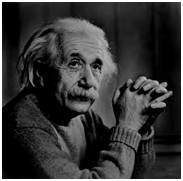
\includegraphics[width=\linewidth]{images/einsteinEscuro.jpg}
	  \caption{Imagem de entrada}
	\endminipage\hspace{1cm}
	\minipage{0.30\textwidth}
	  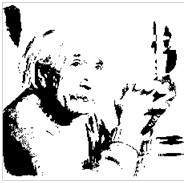
\includegraphics[scale=0.62]{images/claro.jpg}
	  \caption{Imagem de saída}
	\endminipage
\end{figure}

\subsubsection{Transformação Gamma - Power Law - Exponencial}
Nesse caso, também há a transformações de exponenciação e de radiciação. Essa transformação é representada a partir da fórmula:
\\
\large{\textcolor{red}{AQUI A TRANSFORMAÇÃO GAMMA É \\ $g(f(x,y)) = c \cdot f(x,y)^{\gamma}$ OU $g(f(x,y)) = c \cdot f(x,y)^{\dfrac{1}{\gamma}}$ ???}}
\begin{center}
	$g(f(x,y)) = c \cdot f(x,y)^{\dfrac{1}{\gamma}}$
\end{center}
Observe exemplos dessas transformações:
\begin{figure}[!htb]
	\centering
	\minipage{0.25\textwidth}
	  	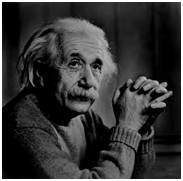
\includegraphics[width=\linewidth]{images/einsteinEscuro.jpg}
	  	\caption{$\gamma = 10$}
	\endminipage\hspace{1cm}
	\minipage{0.25\textwidth}
		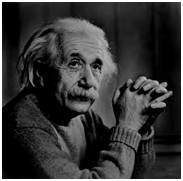
\includegraphics[width=\linewidth]{images/einsteinEscuro.jpg}
		\caption{$\gamma = 8$}
  	\endminipage\hspace{1cm}
	\minipage{0.25\textwidth}
	  	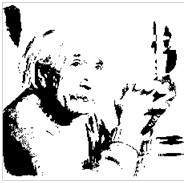
\includegraphics[width=\linewidth]{images/claro.jpg}
	  	\caption{$\gamma = 6$}
	\endminipage
\end{figure}

\section{Conceito de Convolução}
Convolução é uma tereira maneira de manipular imagens. Já abordamos transformações em histogramas e funções de transformação grascale. Matemáticamente, 
convolução pode ser representado como:
\begin{center}
	$g(x, y) = h(x,y) * f(x,y)$
\end{center}
Podemos dizer que a ``máscara'' envolveu a imagem.
Por outro, lado, devido à comutatividade dessa operação, podemos escrever:
\begin{center}
	$g(x, y) = f(x,y) * h(x,y)$
\end{center}
Que pode se explicado dizendo que a imagem foi envolvida pela ``máscara''. $h(x,y)$ é a máscara, ou filtro.

\subsection{Máscara}
A máscara pode ser interpretada, também, como um sinal. Representada através de uma matriz bidimensional, a máscara deve ser quadradada e ter dimensões 
ímpares.

\subsubsection{Como efetuar convolução utilizando a máscara}
Seja a seguinte matriz uma representação de nossa máscara:
\begin{center}
	$
	\begin{bmatrix}
		1 & 2 & 3 \\
		4 & 5 & 6 \\
		7 & 8 & 9 \\
	\end{bmatrix}	
	$
\end{center}
Primeiro, devemos espelhar a matriz horizontalmente:
\begin{center}
	$
	\begin{bmatrix}
		3 & 2 & 1 \\
		6 & 5 & 4 \\
		9 & 8 & 7 \\
	\end{bmatrix}	
	$
\end{center}
Segundo, devemos espelhar a matriz verticalmente:
\begin{center}
	$
	\begin{bmatrix}
		9 & 8 & 7 \\
		6 & 5 & 4 \\
		3 & 2 & 1 \\
	\end{bmatrix}	
	$
\end{center}
Agora, vamos considerar que nossa imagem seja representada pela seguinte matriz:
\begin{center}
	$
	\begin{bmatrix}
		2   & 4   & 6 \\
		8   & 10  & 12 \\
		14  & 16  & 18 \\
	\end{bmatrix}	
	$
\end{center}
Por fim, para efetuar a convolução, devemos pegar a máscara, guiada pelo seu elemento central, e ``colocá-la'' sobre cada elemento da imagem. 
Ao fazer isso, devemos multiplicar os elementos que se sobrepõe e efetuar a soma dessas multiplicações. Depois disso, o resultado obtido deve ser 
colocado na posição que estamos analisando. Por exemplo: Ao colocarmos a máscara sobre o elemento de índice $(0, 0)$ da 
imagem --- nesse exemplo ---, os elementos que se sobreporiam 
seriam os seguintes: $5$ sobre o $2$, $4$ sobre $4$, $1$ sobre o $10$ e $2$ sobre o $8$. Efetuando as multiplicações e as somas teríamos: 
$5 \cdot 2 + 4 \cdot 4 + 1 \cdot 10 + 2 \cdot 8 = 10 + 16 + 10 + 16 = 52$. O valor $52$ deve ser colocado na posição do índice em questão.

\subsubsection{Vantagens da Convolução}
Com convulução podemos realizar feitos que não são possíveis com os demais métodos comentados. Por exemplo:
\begin{itemize}
	\item Redução de ruídos
 	\item Detecção de bordas
 	\item blurring
 	\item Sharpening
\end{itemize}

\section{Conceito de Máscara}
Uma máscara nada mais é que um filtro que é aplicado na imagem, de ponto a ponto, como mostrado na seção anterior. A cada ponto, a resposta do filtro 
é calculada a partir de uma relação pré-definida. De forma geral, há dois tipos principais de filtros: filtros lineares e filtros de domínio de frequência 
--- frequency domain filters. Os usos mais comuns dos filtros são: blurring, sharpening, detecção de bordas e redução de ruídos.
\\

Redução de ruído e blurring estão relacionados. Para ``borrar'' uma imagem, usamos máscaras para fazer com que, haja uma transição suave entre pixels de 
valores diferentes. Desse modo, a redução de ruído é feita utilizando blurring. Além disso, as máscaras são usadas para detectar e deixar as bordas mais 
``afiadas'' (sharpening). Observe uma imagem após a plicação desse efeito:

\begin{figure}[!htbp]
	\centering
	\minipage{0.30\textwidth}
	  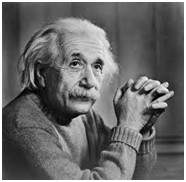
\includegraphics[width=\linewidth]{images/einstein256.jpg}
	  \caption{Imagem de entrada}
	\endminipage\hspace{1cm}
	\minipage{0.30\textwidth}
	  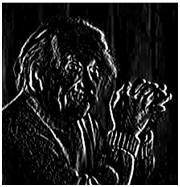
\includegraphics[scale=0.62]{images/bordas.jpg}
	  \caption{Imagem de saída}
	\endminipage
\end{figure}

\section{Conceito de Blurring}
Para borrar ou esfumaçar uma imagem, comumente utilizamos os seguintes tipos de filtros: filtro de média, filtro de média ponderada e filtro gaussiano. 
Focaremos nos dois primeiros.
\\
\begin{enumerate}
	\item Filtro de Média:
	\\
	Aqui, a ideia é realizar fazer com que o elemento sobre o qual aplicaremos o filtro tenha o valor da média aritmética de sua vizinhança.
	para fazer isso, produzimos uma máscara de dimensões $n \times n$ com $n$ ímpar tal que, todos os elementos sejam iguais e sua soma seja igual à 
	$1$. Dessa maneira, ao efetuarmos a convolução, digamos em um pixel no meio da imagem, esse pixel será equivalente ao 
	valor da média aritmética dos $n^2$ elementos mais próximos a ele (incluindo ele próprio). Observe algumas imagens que foram submetidas à esse processo:
	\\
	\begin{figure}[!htb]
		\centering
		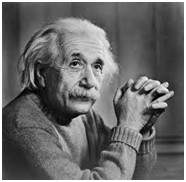
\includegraphics[scale=0.62]{images/einstein256.jpg}
		\caption{Imagem original}
	\end{figure}
	\begin{figure}[!htb]
		\centering
		\minipage{0.30\textwidth}
		  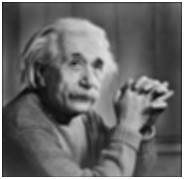
\includegraphics[width=\linewidth]{images/borrado5.jpg}
		  \caption{Filtro $5 \times 5$}
		\endminipage\hspace{1cm}
		\minipage{0.30\textwidth}
		  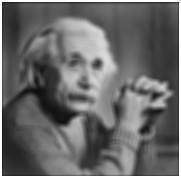
\includegraphics[scale=0.62]{images/borrado7.jpg}
		  \caption{Filtro $7 \times 7$}
		\endminipage
	\end{figure}

	\begin{figure}[!htb]
		\centering
		\minipage{0.30\textwidth}
		  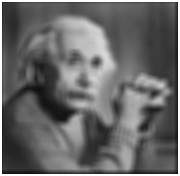
\includegraphics[width=\linewidth]{images/borrado9.jpg}
		  \caption{Filtro $9 \times 9$}
		\endminipage\hspace{1cm}
		\minipage{0.30\textwidth}
		  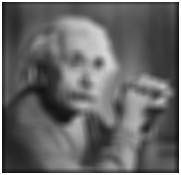
\includegraphics[width=\linewidth]{images/borrado11.jpg}
		  \caption{Filtro $11 \times 11$}
		\endminipage
	\end{figure}

	\item Filtro de Média Ponderada:
 	\\
	Nesse caso, a ideia é parecida com a mostrada no ítem anterior, contudo, teremos um peso maior associado aos elementos centrais, certificando que 
	as propriedades da soma dos elementos na matriz ser $1$, $n$ deve ser ímpar e o peso do elemento central deve ser o maior de todos.
\end{enumerate}


\section{Conceito de bordas - Edges}
Podemos definir ``bordas'' como mudanças bruscas em valores de pixels adjacentes em uma imagem. É interassante ressaltar que estudar como detectar e aprimorar 
as bordas de uma imagem é importante, pois a maior parte da informação das imagens está presente em suas bordas. Então, fazendo isso, podemos fazer a 
imagem ficar mais nítida. Observe um exemplo dessa transformação:

\begin{figure}[!htb]
	\centering
	\minipage{0.30\textwidth}
	  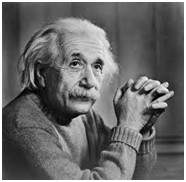
\includegraphics[width=\linewidth]{images/einstein256.jpg}
	  \caption{Imagem original}
	\endminipage\hspace{1cm}
	\minipage{0.30\textwidth}
	  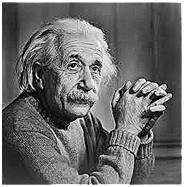
\includegraphics[width=\linewidth]{images/nitido.jpg}
	  \caption{Imagem com o filtro}
	\endminipage
\end{figure}

Nesse sentido, podemos ressaltar os seguintes tipos de bordas: horizontais, verticais e diagonais.
\\

Para fazer isso, são utilizados alguns tipos de filtro:
\begin{itemize}
	\item Prewitt Operator
 	\item Sobel Operator
  	\item Robinson Compass Masks
   	\item Krisch Compass Masks
    \item Laplacian Operator 
\end{itemize}

\subsection{Prewitt Operator}
Essa maneira de encontrar bordas em uma imagem é capaz de detectar bordas horizontais e verticais. Essa, assim como as outras máscaras utilizadas para encontrar 
bordas em imagens, tem seu funcionamento baseado em diferenciação. Nesse sentido, as ``máscaras derivativas'' devem seguir as seguintes propriedades: 
Valores de sinais opostos devem estar presentes na máscara, a soma dos valores deve ser igual a zero e quanto mais peso, mais detecção.
\\

Primeiramente, vamos observar as máscaras que esse método nos fornece. Para detecção na direção vertical, a máscara é a seguinte:
\begin{center}
	$
	\begin{bmatrix}
		-1 & 0 & 1 \\
		-1 & 0 & 1 \\
		-1 & 0 & 1 \\
	\end{bmatrix}
	$
\end{center}
Para entender o funcionamento dessa máscara, pensemos em um exemplo em que a máscara será aplicada no ponto $(x_i, y_j)$ da seguinte imagem/matriz:
\begin{center}
	$
	\begin{bmatrix}
		f(x_{i-1}, y_{j-1}) & f(x_{i-1}, y_j) & f(x_{i-1}, y_{j+1}) \\
		f(x_i, y_{j-1})     & f(x_i, y_j)     & f(x_i, y{j+1})      \\
		f(x_{i+1}, y_{j-1}) & f(x_{i+1}, y_j) & f(x_{i+1}, y_{j+1}) \\
	\end{bmatrix}
	$
\end{center}
Ao aplicarmos essa máscara no ponto referido, $f(x_i, y_j)$ assumirá o valor de:
\begin{center}
\small{$\left(f(x_i, y{j+1}) - f(x_i, y_{j-1})\right) + \left(f(x_{i-1}, y_{j+1}) - f(x_{i-1}, y_{j-1})\right) + \left(f(x_{i+1}, y_{j+1}) - f(x_{i+1}, y_{j-1})\right)$}
\end{center}
Desse modo, como o valor em um pixel será a soma das diferenças (em relação à vertical) dos pixels ao seu redor, se essas diferenças forem grandes, o valor do pixel 
será alto, caso contrário, esse valor será baixo. Cumprindo assim, o papel de aumentar o contraste nas bordas verticais.
\\

O mesmo princípio é utilizado na máscara para detectar as bordas horizontais. A máscara utilizada é:
\begin{center}
	$
	\begin{bmatrix}
	   -1 & -1  & -1 \\
		0 &  0  &  0 \\
		1 &  1  &  1 \\
	\end{bmatrix}
	$
\end{center}
Observe esse método funcionando:
\begin{figure}[!htb]
	\centering
	\minipage{0.25\textwidth}
	  	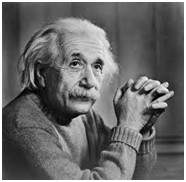
\includegraphics[width=\linewidth]{images/einstein256.jpg}
	  	\caption{Imagem original}
	\endminipage\hspace{1cm}
	\minipage{0.25\textwidth}
		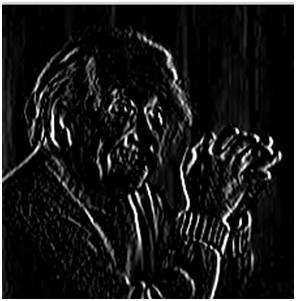
\includegraphics[width=\linewidth]{images/prewittvert.jpg}
		\caption{Detecção de bordas verticais}
  	\endminipage\hspace{1cm}
	\minipage{0.25\textwidth}
	  	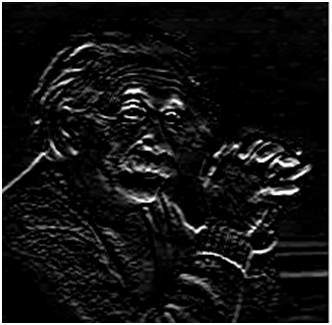
\includegraphics[width=\linewidth]{images/prewitthori.jpg}
	  	\caption{Detecção de bordas horizontais}
	\endminipage
\end{figure}
\subsection{Sobel Operator}
Esse método de realizar detecção de bordas é extremamente similar ao de Prewitt. De maneira análoga, ele é capaz de identificar bordas verticais e horizontais. 
A diferença entre eles é a atribuição de pesos diferentes nesse caso. Contanto que a máscara formada não viole as propriedades das máscaras derivativas.
Um exemplo desse tipo de máscara é:
\\
\begin{center}
	Vertical:
	$
	\begin{bmatrix}
		-1 & 0 & 1 \\
		-2 & 0 & 2 \\
		-1 & 0 & 1 \\
	\end{bmatrix}
	$;
	Horizontal:
	$
	\begin{bmatrix}
	   -1 & -2  & -1 \\
		0 &  0  &  0 \\
		1 &  2  &  1 \\
	\end{bmatrix}
	$
\end{center}
Observe ess método em funcionamento:
\begin{figure}[!htb]
	\centering
	\minipage{0.25\textwidth}
	  	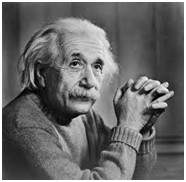
\includegraphics[width=\linewidth]{images/einstein256.jpg}
	  	\caption{Imagem original}
	\endminipage\hspace{1cm}
	\minipage{0.25\textwidth}
		\includegraphics[width=\linewidth]{images/sobelvert.jpg}
		\caption{Detecção de bordas verticais}
  	\endminipage\hspace{1cm}
	\minipage{0.25\textwidth}
	  	\includegraphics[width=\linewidth]{images/sobelhori.jpg}
	  	\caption{Detecção de bordas horizontais}
	\endminipage
\end{figure}
\subsection{Robinson Compass Masks}
Tratando de mais um tipo de máscara derivativa para detectar bordas de imagens, podemos identificar esta como máscara de direção. Isso ocorre pois 
a ideia desta máscara é utilizar uma máscar como as mostradas anteriormente e, simplesmente, rotacioná-la nas $8$ direções de uma bússola. Para fazer isso, 
podemos utilizar qualquer máscara derivativa, observe:
\begin{figure}[!htb]
	\begin{minipage}{.23\linewidth}
	  \centering
	  \[\left[\begin{array}{ccc}
		-1 & 0 & 1 \\
		-2 & 0 & 2 \\
		-1 & 0 & 1
	  \end{array}\right]\]
	  Máscara de direção Norte
	\end{minipage}%
	\begin{minipage}{.23\linewidth}
	  \centering
	  \[\left[\begin{array}{ccc}
		 0 & 1  & 2 \\
		-1 & 0  & 1 \\
		-2 & -1 & 0
	  \end{array}\right]\]
	  Máscara de direção Noroeste
	\end{minipage}
	\begin{minipage}{.23\linewidth}
		\centering
		\[\left[\begin{array}{ccc}
		   1 &  2  &  1 \\
		   0 &  0  &  0 \\
		  -1 & -2  & -1
		\end{array}\right]\]
		Máscara de direção Oeste
	  \end{minipage}
	  \begin{minipage}{.23\linewidth}
		\centering
		\[\left[\begin{array}{ccc}
		   2 &   1   &   0 \\
		   1 &   0   &  -1 \\
		   0 &  -1   &  -2
		\end{array}\right]\]
		Máscara de direção Sudoeste
	  \end{minipage}
\end{figure}

\begin{figure}[!htb]
	\begin{minipage}{.23\linewidth}
	  \centering
	  \[\left[\begin{array}{ccc}
		1 & 0 & -1 \\
		2 & 0 & -2 \\
		1 & 0 & -1
	  \end{array}\right]\]
	  Máscara de direção Sul
	\end{minipage}%
	\begin{minipage}{.23\linewidth}
	  \centering
	  \[\left[\begin{array}{ccc}
		0 & -1  & -2 \\
		1 &  0  & -1 \\
		2 &  1  &  0
	  \end{array}\right]\]
	  Máscara de direção Sudeste
	\end{minipage}
	\begin{minipage}{.23\linewidth}
		\centering
		\[\left[\begin{array}{ccc}
		  -1 &  -2  & -1 \\
		   0 &   0  &  0 \\
		   1 &   2  &  1
		\end{array}\right]\]
		Máscara de direção Leste
	  \end{minipage}
	  \begin{minipage}{.23\linewidth}
		\centering
		$
		\begin{bmatrix*}[l]
		             -2 &            -1   & \phantom{-}  0 \\
		             -1 &  \phantom{-}0   & \phantom{-}  1 \\
		   \phantom{-}0 &  \phantom{-}1   & \phantom{-}  2
		\end{bmatrix*}
		$
		Máscara de direção Nordeste
	  \end{minipage}
  \end{figure}
Disso, temos os seguintes resultados:
\begin{figure}[!htb]
	\centering
	\minipage{0.17\textwidth}
	  	\includegraphics[width=\linewidth]{images/robinson1.jpg}
	  	\caption{Direção Norte}
	\endminipage\hspace{1cm}
	\minipage{0.17\textwidth}
	 	\includegraphics[width=\linewidth]{images/robinson2.jpg}
	  	\caption{Direção Noroeste}
	\endminipage\hspace{1cm}
	\minipage{0.17\textwidth}
		\includegraphics[width=\linewidth]{images/robinson3.jpg}
		\caption{Direção Oeste}
  	\endminipage\hspace{1cm}
  	\minipage{0.17\textwidth}
  		\includegraphics[width=\linewidth]{images/robinson4.jpg}
  		\caption{Direção Sudoeste}
	\endminipage
\end{figure}
\begin{figure}[!htb]
	\centering
	\minipage{0.17\textwidth}
	  	\includegraphics[width=\linewidth]{images/robinson5.jpg}
	  	\caption{Direção Sul}
	\endminipage\hspace{1cm}
	\minipage{0.17\textwidth}
	 	\includegraphics[width=\linewidth]{images/robinson6.jpg}
	  	\caption{Direção Sudeste}
	\endminipage\hspace{1cm}
	\minipage{0.17\textwidth}
		\includegraphics[width=\linewidth]{images/robinson7.jpg}
		\caption{Direção Leste}
  	\endminipage\hspace{1cm}
  	\minipage{0.17\textwidth}
  		\includegraphics[width=\linewidth]{images/robinson8.jpg}
  		\caption{Direção Nordeste}
	\endminipage
\end{figure}
\subsection{Krisch Compass Masks}
Esse método é muito similar ao de Robinson. A diferença, é que já possuímos valores dá máscara que será rotacionada:

\begin{figure}[!htb]
	\begin{minipage}{.23\linewidth}
	  \centering
	  \[\left[\begin{array}{ccc}
		-3 & -3 & 5 \\
		-3 &  0 & 5 \\
		-3 & -3 & 5
	  \end{array}\right]\]
	  Máscara de direção Norte
	\end{minipage}%
	\begin{minipage}{.23\linewidth}
	  \centering
	  \[\left[\begin{array}{ccc}
		-3 &  5  &  5 \\
		-3 &  0  &  5 \\
		-3 & -3  & -3
	  \end{array}\right]\]
	  Máscara de direção Noroeste
	\end{minipage}
	\begin{minipage}{.23\linewidth}
		\centering
		\[\left[\begin{array}{ccc}
		   5 &  5  &  5 \\
		  -3 &  0  & -3 \\
		  -3 & -3  & -3
		\end{array}\right]\]
		Máscara de direção Oeste
	  \end{minipage}
	  \begin{minipage}{.23\linewidth}
		\centering
		\[\left[\begin{array}{ccc}
		   5 &   5   &  -3 \\
		   5 &   0   &  -3 \\
		  -3 &  -3   &  -3
		\end{array}\right]\]
		Máscara de direção Sudoeste
	  \end{minipage}
\end{figure}

\begin{figure}[!htb]
	\begin{minipage}{.23\linewidth}
	  \centering
	  \[\left[\begin{array}{ccc}
		5 &  -3 &  -3 \\
		5 &   0 &  -3 \\
		5 &  -3 &  -3
	  \end{array}\right]\]
	  Máscara de direção Sul
	\end{minipage}%
	\begin{minipage}{.23\linewidth}
	  \centering
	  \[\left[\begin{array}{ccc}
	   -3 & -3  & -3 \\
		5 &  0  & -3 \\
		5 &  5  & -3
	  \end{array}\right]\]
	  Máscara de direção Sudeste
	\end{minipage}
	\begin{minipage}{.23\linewidth}
		\centering
		\[\left[\begin{array}{ccc}
		  -3 &  -3  & -3 \\
		  -3 &   0  & -3 \\
		   5 &   5  &  5
		\end{array}\right]\]
		Máscara de direção Leste
	  \end{minipage}
	  \begin{minipage}{.23\linewidth}
		\centering
		$
		\begin{bmatrix*}[l]
		             -3 &            -3   &             -3 \\
		             -3 &  \phantom{-}0   & \phantom{-}  5 \\
		             -3 &  \phantom{-}5   & \phantom{-}  5
		\end{bmatrix*}
		$
		Máscara de direção Nordeste
	  \end{minipage}
  \end{figure}
  Observe os resultados em uma imagem real:
  \begin{figure}[!htbp]
	\centering
	\minipage{0.17\textwidth}
	  	\includegraphics[width=\linewidth]{images/kirsch2.jpg}
	  	\caption{Direção Norte}
	\endminipage\hspace{1cm}
	\minipage{0.17\textwidth}
	 	\includegraphics[width=\linewidth]{images/kirsch3.jpg}
	  	\caption{Direção Noroeste}
	\endminipage\hspace{1cm}
	\minipage{0.17\textwidth}
		\includegraphics[width=\linewidth]{images/kirsch4.jpg}
		\caption{Direção Oeste}
  	\endminipage\hspace{1cm}
  	\minipage{0.17\textwidth}
  		\includegraphics[width=\linewidth]{images/kirsch5.jpg}
  		\caption{Direção Sudoeste}
	\endminipage
\end{figure}
\begin{figure}[!htbp]
	\centering
	\minipage{0.17\textwidth}
	  	\includegraphics[width=\linewidth]{images/kirsch6.jpg}
	  	\caption{Direção Sul}
	\endminipage\hspace{1cm}
	\minipage{0.17\textwidth}
	 	\includegraphics[width=\linewidth]{images/kirsch7.jpg}
	  	\caption{Direção Sudeste}
	\endminipage\hspace{1cm}
	\minipage{0.17\textwidth}
		\includegraphics[width=\linewidth]{images/kirsch8.jpg}
		\caption{Direção Leste}
  	\endminipage\hspace{1cm}
  	\minipage{0.17\textwidth}
  		\includegraphics[width=\linewidth]{images/kirsch9.jpg}
  		\caption{Direção Nordeste}
	\endminipage
\end{figure}
\vspace{3cm}
\subsection{Laplacian Operator}
Por fim, temos o método de Laplace para encontrar bordas de imagens. Diferentemente dos outros, que eram métodos que se baseavam em primeiras derivadas, 
este utiliza uma máscara derivativa de segunda ordem. Nesse sentido, temos somente dois tipos de máscaras de Laplace: Positiva (detecta bordas externas) e 
Negativa (detecta bordas internas).
Primeiro, observe essas duas máscaras de Laplace:
\begin{center}
	Positiva:
	$
	\begin{bmatrix}
		0 &  1  & 0 \\
		1 & -4 & 1 \\
		0 &  1  & 0 \\
	\end{bmatrix}
	$;
	Negativa:
	$
	\begin{bmatrix}
	    0 &  -1  &   0 \\
	   -1 &   4  &  -1 \\
		0 &  -1  &   0 \\
	\end{bmatrix}
	$
\end{center}
Um detalhe importante, é que, para obter o resultado esperado, não basta realizar a convolução na imagem utilizando essa máscara. Na realidade, 
se aplicarmos a máscara positiva em uma imagem, teremos de subtrair a imagem resultante da imagem original. Já se aplicarmos a máscara negativa, 
teremos de adicionar a imagem resultante à imagem original.

Observe os resultados:
\begin{figure}[!htb]
	\centering
	\minipage{0.26\textwidth}
	  	\includegraphics[width=\linewidth]{images/einstein256.jpg}
	  	\caption{Imagem original}
	\endminipage\hspace{1cm}
	\minipage{0.25\textwidth}
		\includegraphics[width=\linewidth]{images/laplacian1.jpg}
		\caption{Detecção de bordas externas}
  	\endminipage\hspace{1cm}
	\minipage{0.25\textwidth}
	  	\includegraphics[width=\linewidth]{images/laplacian2.jpg}
	  	\caption{Detecção de bordas internas}
	\endminipage
\end{figure}
\section{Análise do Frequência de Domínio - Frequency Domain Analysis}
Até agora, analisamos os sinais obtidos em respeito do tempo ou do espaço. Ou seja, geralmente, o tempo ou a posição são as variáveis independentes. 
Nesse caso, a frequência se torna o domínio da função. Agora lidaremos com a medida de mudança de valores dos pixels. Nesse sentido, 
o processo de transformação na imagem segue os seguintes passos:
\begin{itemize}
	\item Recebemos uma imagem como entrada.
 	\item Convertemos essa imagem para sua distribuição de frequências.
  	\item Processamos essa distribuição.
   	\item Convertemos a nova distribuição em uma nova imagem.
    \item Entregamos a imagem de saída.
\end{itemize}

\textcolor{red}{\large{DIFÍCIL NÃO ENTENDI AS APLICAÇÕES E ACHEI MAL EXPLICADO}
\section{Series e Transformadas de Fourier}
\section{Series de Fourier}
A ideia das series de Fourier é simplesmente que um sinal pode ser decomposto como uma soma infinita de senos e cossenos multiplicados por constantes.
Assim, ao tratarmos sobre Transformadas de Fourier desejamos decompôr o sinal (imagem) em senos e cossenos, e a saída dessa transformada é a representação 
da imagem cujo domínio são as frequências. Faremos uma breve explicação sobre transformadas de Fourier discretas (DFT) --- a aplicação em imagens digitais, 
devido à quantização e amostragem.
\\
Assim, o número de frequências corresponderá ao número de pixels. Desse modo, para uma imagem quadrada $N \times N$, a transformada discreta de Fourier, 
que converte uma imagem para a sua representação que possui frequência como domínio, é dada por:
\begin{center}
	\[F(u,v) = \dfrac{1}{N^2} \sum_{x = 0}^{N-1} \sum_{y=0}^{N-1} f(x,y)e^{-j2\pi\left(\dfrac{ux}{N} + \dfrac{vy}{N}\right)}\]
\end{center}
A transformada inversa de Fourier, que converte a imagem à sua forma original é dada por:
\begin{center}
	\[f(x,y) = \sum_{x = 0}^{N-1} \sum_{y=0}^{N-1} F(u,v)e^{j2\pi\left(\dfrac{ux}{N} + \dfrac{vy}{N}\right)}\]
\end{center}
}
\textcolor{red}{\large{ACHEI MAL EXPLICADO}
\section{Teorema da Convulução}
O teorema da convulução serve para relacionar uma imagem à sua representação no domínio das frequências. Observe a representação gráfica dessas duas 
interpretações de uma imagem:}
\begin{figure}[!htb]
	\centering
	\minipage{0.30\textwidth}
	  \includegraphics[width=\linewidth]{images/einstein256.jpg}
	  \caption{Imagem original}
	\endminipage\hspace{1cm}
	\minipage{0.30\textwidth}
	  \includegraphics[width=\linewidth]{images/freq.jpg}
	  \caption{Imagem com o filtro}
	\endminipage
\end{figure}

\textcolor{red}{
O Teorema da Convolução pode ser representado como:
\begin{center}
 $f(x,y) * h(x,y) \Leftrightarrow F(u,v)H(u,v)$
 \\
 $f(x,y)h(x,y) \Leftrightarrow F(u,v)*H(u,v)$
 \\
 $h(x,y) \Leftrightarrow H(u,v)$
\end{center}
Ou seja, realizar convolução tendo o espaço como domínio é equivalente à filtrar tendo as frequências como domínio, e vice-versa.
}
\textcolor{red}{
\section{Filtros Passa Alta e Filtros Passa Baixa em Imagens}}


\section{Introdução aos Espaços de Cor}
Alguns dos padrões de cores utilizados atualmente são:
\begin{itemize}
	\item RGB
 \item CMYK
 \item YUV
 \item YIQ
 \item YCbCr
\end{itemize}

Sobre RGB, sabemos que é um modelo de cor extremamente utilizado. A representação das imagens utilzando esse formato passa a consistir em uma matriz 
3D, em que, cada pixel possui $3$ valores --- R, G e B --- , ou, também podemos interpretar como $3$ matrizes distintas.

No modelo CMYK, já foi abordado que podemos tratar, separadamente CMY e K, e que esse é um padrão comumente utilzado em impressoras. Para converter RGB 
para CMY, fazemos: 
\begin{center}
	$
	\begin{bmatrix}
		C \\
		M \\
		Y
	\end{bmatrix}
	= 
	\begin{bmatrix}
		2^{bpp} - 1 \\
		2^{bpp} - 1 \\
		2^{bpp} - 1
	\end{bmatrix}
	- 
	\begin{bmatrix}
		R \\
		G \\
		B
	\end{bmatrix}
	$
\end{center}
Sobre YUV, podemos dizer que é utilizado nos seguintes padrões de cor:
\begin{itemize}
	\item NTSC (National Television System Committee)
 	\item PAL (Phase Alternating Line)
 	\item SECAM (Sequential couleur a amemoire, French for “sequential color with memory)
\end{itemize}
Já em relação ao YCbCr, é interessante ressaltar que é utilizado, principalmente, na compressão de JPEG e MPEG.

\textcolor{red}{
\section{Introdução à Compressão de JPEG}}

\section{Reconhecimento Ótico de Caracteres - OCR}
OCR consiste na conversão de textos (manuscritos, escaneados, fotografados) para textos compreensíveis para o computador. OCR revolucionou os mais 
diversos tipos de indústrias ao redor do mundo, principalmente na qeustão de documentos. Entre diversas aplicações importantes dessa tecnologia, 
podemos ressaltar as seguintes:
\begin{itemize}
	\item Bancos (principalmente em relação à cheques)
 \item Auxílio à pessoas com deficiências visuais
 \\
 Com OCR, existe a possibilidade de que o computador efetue leitura convencional (sem ser braile) para essas pessoas.

 \item Vendas --- Recinhecimento de caracteres em códigos de barra
\end{itemize}

\section{Visão Computacional}
Visão Computacional busca replicar a visão humana utilizando computadores. Há uma hierarquia no estudo de visão computacional:
\begin{itemize}
	\item Baixo nível:
	\\
	Inclui processamento da imagem para futura extração
	\item Nível Intermediário:
 	\\
	Inclui econhecimento de objetos e interpretação de cenas
	\item Nível alto:
 	\\
	Inclui descrição conceitual de cenas.
\end{itemize}
Alguns dos incontáveis exemplos de aplicação dessa área de estudo são:
\begin{itemize}
	\item Robótica:
 	\\
	Carros inteligentes que desviam de objetos, interação entre robôs e humanos, movimentação de robôs utilizando visão computacional e inteligência 
	artificial.
	\item Medicina:
	\\
	Classificação de doenças usando imagens médicas, cirurgias guiadas por robôs, construção de representação de órgãos para realizar exames.
	\item Indústria:
	\\
	Reconhecimento de padrões como OCR, ordenação de objetos utilizando visão computacional, interpretação de documentos.
\end{itemize}



\section{Computação Gráfica}
Esse tipo tipo de computação foca na criação, manipulação e renderização de objetos e suas imagens relacionadas. Depois do crescimento da 
indústria dos vídeo games, essa área se expandiu consideravelmente. Nesse sentido, as tarefas relacionadas à ela são realizadas, geralmente, com 
o auxílio de hardware e software especializados. Um exemplo claro disso são as poderosíssimas placas de vídeo que surgem ano após ano.
Alguns exemplo de atuação dessas tecnologias são:
\begin{itemize}
	\item Design
 	\\ Utilizado para fazer modelos 3D e realistas de edifícios, carros, aviões, etc.
 	\item Animação 3D e Vídeo games
 	\item Educação
 	\\
 Utilizado para gerar modelos de corpos para auxiliar no estudo da medicina, por exemplo. Ou simulações para pilotos de avião.
\end{itemize}

\end{document}






